% !TEX root = ../patchEmbeddings_review.tex

\section{Related work} \label{sec:related_work}
\TODO{restructure, to be rewritten}

\textbf{Proposal-based methods} have been highly successful in instance segmentation competitions like MS COCO \cite{lin2014microsoft}, Pascal VOC2012 \cite{everingham2010pascal} and CityScapes \cite{cordts2016cityscapes}. They decompose the instance segmentation task into two steps that consists in generating object proposals and assigning to each bounding box a class and a binary segmentation mask \cite{he2017mask,porzi2019seamless,liu2018path,yang2012layered,li2017fully,ladicky2010and,hariharan2014simultaneous,chen2015multi,dai2016instance,liang2016reversible}. 
% They commonly rely on {Faster-RCNN}~\cite{ren2015faster} and can be trained end-to-end using non-maximum suppression. 
Other methods use instead recurrent models to sequentially generate instances one-by-one \cite{romera2016recurrent,ren2017end}.

\begin{figure}[t]
\centering
        % \includegraphics[width=0.4\textwidth,trim=0.25in 0.25in 0.68in 0.36in,clip]{./figs/SSBM_experiments.pdf} % 0.45
        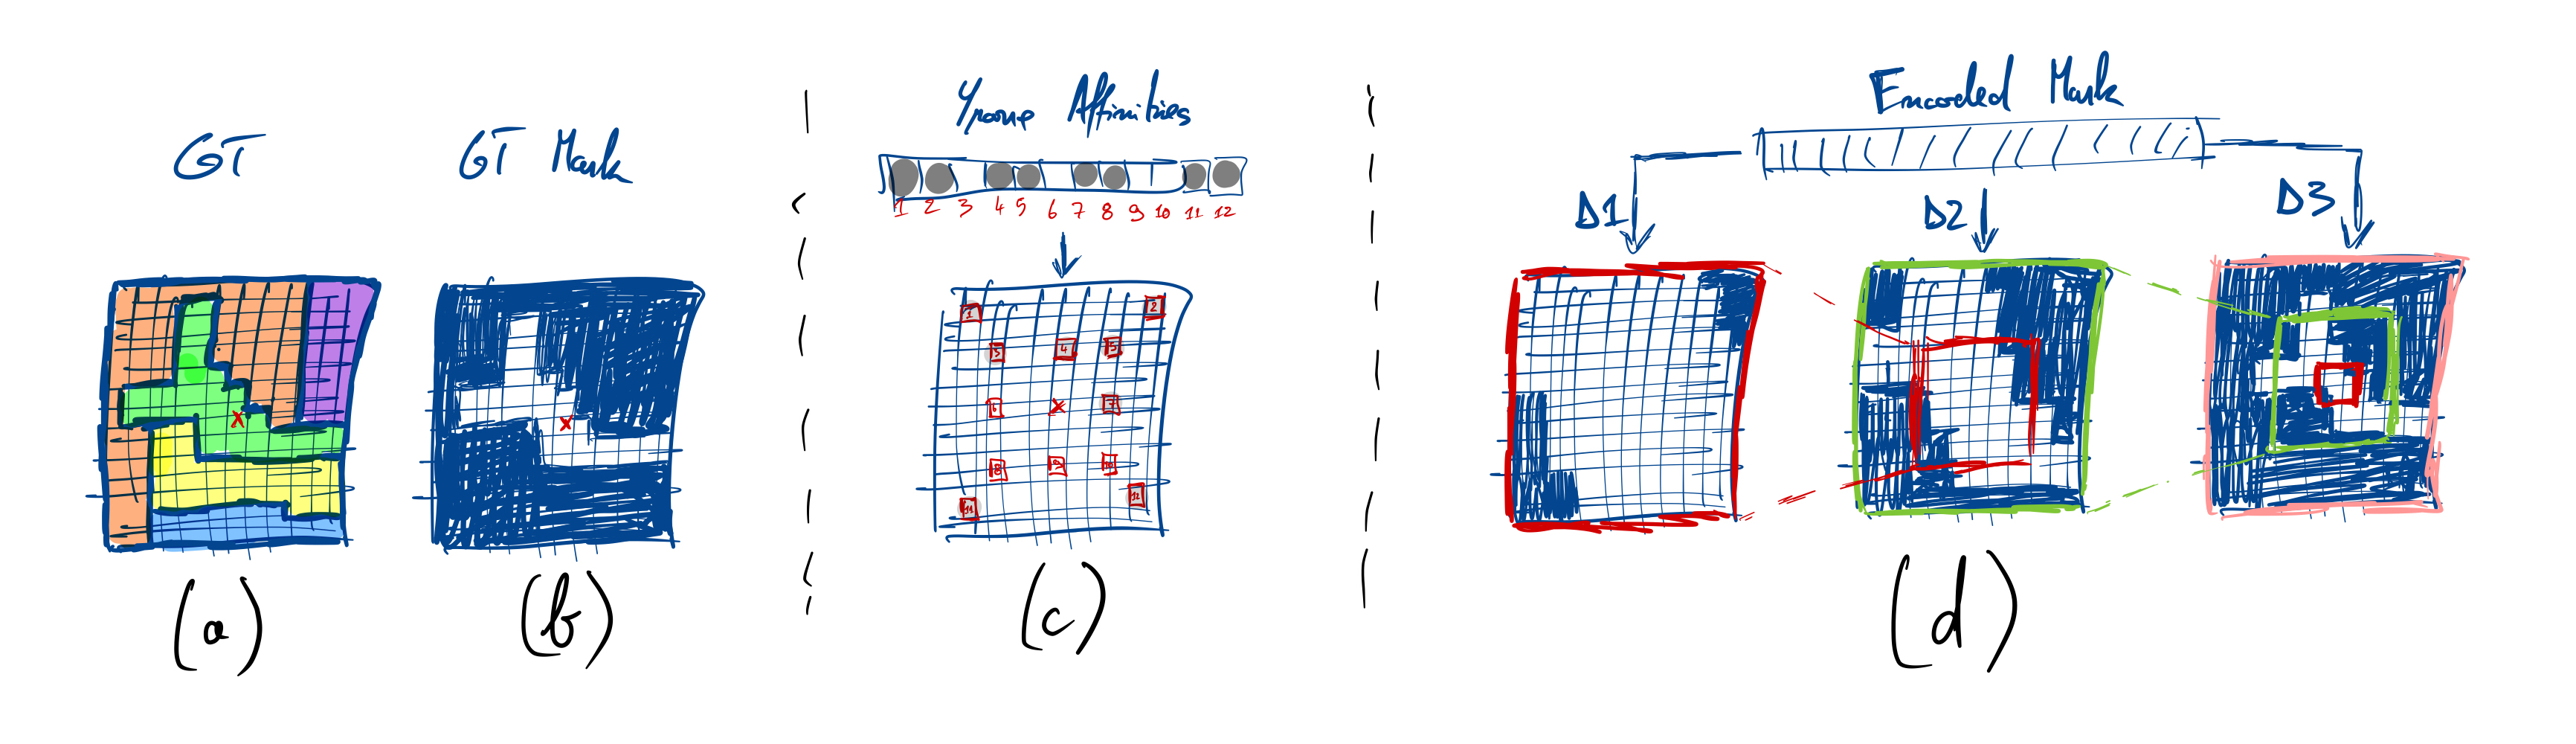
\includegraphics[width=\textwidth]{./figs/masks_explained.jpg} % 0.45
        \caption{Comparison between sparse affinities and encoded probability masks...}
    \label{fig:comparing_masks_affs}
\end{figure}


\textbf{Proposal-free methods} adopt a bottom-up approach by directly grouping pixels into instances. Recently, there has been a growing interest for such  methods that do not involve object detection, since, in certain types of data, object instances cannot be approximated by bounding boxes. For example, the approach proposed in \cite{kirillov2017instancecut} uses a combinatorial framework for instance segmentation, 
% SGN \cite{liu2017sgn} sequentially group pixels into lines and then instances;
whereas a watershed transform is learned in \cite{bai2017deep} by also predicting its gradient direction. 
% whereas the template matching \cite{uhrig2016pixel} deploys scene depth information.
Others use metric learning to predict high-dimensional associative pixel embeddings that map pixels of the same instance close to each other, while mapping pixels belonging to different instances further apart \cite{lee2019learning,fathi2017semantic,newell2017associative,de2017semantic}. % kulikov2018instance
Final instances are then retrieved by applying a clustering algorithm, like in the end-to-end trainable mean-shift pipeline of \cite{kong2018recurrentPix}. 
Other recent successful methods simply let the model predict the relative coordinates of the instance center \cite{neven2019instance,cheng2019panopticdeeplab} or, given a point $(x,y)$ in the image, they train a model to generate the mask of the instance located at $(x,y)$ \cite{sofiiuk2019adaptis}. 

\textbf{Edge detection} also experienced recent progress thanks to deep learning, both on natural images \cite{Gao_2019_ICCV,liu2018affinity,xie2015holistically,kokkinos2015pushing} and biological data \cite{lee2017superhuman,schmidt2018cell,meirovitch2016multi,ciresan2012deep}. In neuron segmentation for connectomics, a field of neuroscience we also address in our experiments, boundaries are converted to final instances with subsequent postprocessing and superpixel-merging:
some use loopy graphs \cite{kaynig2015large,krasowski2015improving} or trees \cite{meirovitch2016multi,liu2016sshmt,liu2014modular,funke2015learning,uzunbas2016efficient} to represent the region merging hierarchy; the lifted multicut \cite{beier2017multicut} formulates the problem in a combinatorial framework, whereas 
flood-filling networks \cite{januszewski2018high} and MaskExtend \cite{meirovitch2016multi} use a CNN to iteratively grow one region/neuron at the time; recently, the work of \cite{meirovitch2019cross} made the process more efficient by employing a combinatorial encoding of the segmentation.
A structured learning approach was also proposed in \cite{funke2018large,turaga2009maximin}.

\TODO{}
 average linkage \cite{liu2018affinity,lee2017superhuman}, linkage learned by a random forest classifier \cite{nunez2013machine,knowles2016rhoananet}.


Extra approaches based signed graphs: Modern integer linear programming solvers can tackle problems of considerable size \cite{andres2012globally}, but accurate approximations \cite{pape2017solving,beier2016efficient,yarkony2012fast}, greedy agglomerative algorithms \cite{levinkov2017comparative,wolf2019mutex,keuper2015efficient,kardoostsolving} and persistence criteria \cite{lange2018partial,lange2018combinatorial} have been proposed for even larger graphs. 


proposal-free methods \cite{liu2018affinity,wolf2018mutex,lee2017superhuman} to predict long-range relationships between pixels.

\TODO{} patchPerPix, embeddings on connectomics, SSAP


